\documentclass[aip,apl,reprint]{revtex4-1}
\usepackage{graphicx}
\usepackage{bm}

\begin{document}

\title{Propagation length of mid-infrared surface plasmon polaritons at gold/air interface}
\author{Nobuyoshi Hiramatsu}
%\author{N. Hiramatsu}
\altaffiliation[Also at ]{Department of Applied Physics, Faculty of Engineering, the University of Tokyo, 7-3-1 Hongo, Bunkyo-ku, Tokyo 113-8656, Japan}
\affiliation{Institute of Industrial Science, the University of Tokyo, 4-6-1 Komaba, Meguro-ku, Tokyo 153-8505, Japan}
\author{Fumiya Kusa}
%\author{F. Kusa}
\affiliation{Institute of Industrial Science, the University of Tokyo, 4-6-1 Komaba, Meguro-ku, Tokyo 153-8505, Japan}
\author{Akinobu Takegami}
%\author{A. Takegami}
\affiliation{Institute of Industrial Science, the University of Tokyo, 4-6-1 Komaba, Meguro-ku, Tokyo 153-8505, Japan}
\author{Kotaro Imasaka}
%\author{K. Imasaka}
\affiliation{Institute of Industrial Science, the University of Tokyo, 4-6-1 Komaba, Meguro-ku, Tokyo 153-8505, Japan}
\author{Ikki Morichika}
%\author{I. Morichika}
\affiliation{Institute of Industrial Science, the University of Tokyo, 4-6-1 Komaba, Meguro-ku, Tokyo 153-8505, Japan}
\author{Jumpei Tayama}
%\author{J. Tayama}
\affiliation{Institute of Industrial Science, the University of Tokyo, 4-6-1 Komaba, Meguro-ku, Tokyo 153-8505, Japan}
\author{Satoshi Ashihara}
%\author{S. Ashihara}
%\thanks{Corresponding author.}
\email{ashihara@iis.u-tokyo.ac.jp}
\affiliation{Institute of Industrial Science, the University of Tokyo, 4-6-1 Komaba, Meguro-ku, Tokyo 153-8505, Japan}

\date{\today}

\begin{abstract}
We measured the propagation length of mid-infrared surface plasmon polaritons (SPPs) at gold/air interface, and correlated the SPP propagation length with the surface morphology of gold. We confirmed that SPPs at gold/air interface propagate for a distance as long as $>10\:\mathrm{mm}$ at a wavelength of $10.6\:\mathrm{\mu m}$, in good agreement with the value predicted from the dielectric constant of polycrystalline gold. We demonstrated that the SPP propagation length increases by thermal annealing treatment, accompanied by the increased grain size and the suppressed surface roughness. Quantitative evaluation of the SPP propagation length is important in designing plasmonic devices and beneficial for deeper understandings of the loss mechanism and the achievable electric-field enhancements.
\end{abstract}

\maketitle
 
\section{Introduction}
Plasmonics in the mid-infrared (IR) range has gained increasing attention\cite{Stanley, Law}, because of potential applications to surface-enhanced spectroscopy\cite{Neubrech, Hoang}, chemical/bio sensing\cite{Cleary2008}, thermal radiation control\cite{Kusunoki}, optoelectronic circuit\cite{Ebbesen, Soref}, nonlinear light-matter interactions\cite{Kusa2015}, etc. Surface plasmons (SPs), including surface plasmon polaritons (SPPs) and localized surface plasmons (LSPs), can be excited at mid-IR wavelengths on various materials, such as noble metals, highly-doped semiconductors, graphene, etc\cite{Law}. The behaviors of SPs, however, significantly vary according to the material where they are excited. 

On highly-doped semiconductors and graphenes with plasma frequencies in mid-IR \cite{Law}, SPs are closely bound to the material surface, exhibiting wavelength shortening and large Ohmic loss at mid-IR wavelengths. Therefore, these materials are suited for achieving subwavelength confinement. On noble metals with plasma frequencies in visible, on the other hand,
 SPs are weakly bound to the material surface, exhibiting subtle wavelength shortening and small Ohmic loss at mid-IR wavelengths . Therefore noble metals are advantageous in applications where any of small loss, long propagation length, and large electric-field enhancement is required \cite{Law, Kusa2014}.

Propagation length of SPPs is an important physical quantity that characterizes materials for plasmonics. First, it sets the upper limit of the device size in applications of sensors and optoelectronic circuits. Second, it is a direct measure of the Ohmic loss, which underlies the degree of electric-field enhancement upon SP excitation. Here we note that electric-field enhancement plays key roles in many plasmonic applications. 

In general, SP oscillation decays by radiatjkive damping and irradiative damping\cite{Link}, the latter of which corresponds to the Ohmic loss and is reflected in the dielectric constant of material. Radiative damping occurs by coupling with free-propagating light, and its rate strongly depends on size and shape of each metal structure. The Ohmic loss originates from scattering of free electrons by electrons, phonons, defects, impurities, surface roughness, grain boundaries, etc., and is more inherent to each material. Therefore, evaluation of SPP propagation length, together with characterization of material morphology, helps us understand the physics behind the Ohmic loss.

Among noble metals, gold is an excellent plasmonic material, because of its high metallic conductivity and superior chemical stability\cite{Zayats}. Although there have been a report on the propagation length of mid-IR SPPs at copper/air interface\cite{Shiba}, a report on the propagation length of visible SPPs at gold/air interface\cite{Kuttge}, and investigations on IR dielectric function of gold in relation to surface morphology\cite{Trollmann, Olmon}, there has been no report, to the best of our knowledge, on the propagation length of mid-IR SPPs at gold/air interface.

In this study, we experimentally measure the propagation length of SPPs at gold/air interface at a mid-IR wavelength of $10.6\:\mathrm{\mu m}$. We showed that the SPPs propagate for a distance about $10\:\mathrm{mm}$, in agreement with the value predicted from the dielectric constant of polycrystalline gold. In addition, we correlated the SPP propagation length with surface morphology, which was controlled by thermal annealing and characterized by atomic force microscopy (AFM). Then, the SPP propagation length was demonstrated to increase by the simple treatment of thermal annealing, accompanied by increased grain size and suppressed surface roughness.

\section{Device design and fabrication}
\label{sec:device}
In order to measure the propagation length of SPPs, we designed a series of SPP waveguide devices. Each device consists of an input coupler, an SPP waveguide, and an output coupler.  The input and output couplers are surface relief gratings made of gold. SPPs are  excited at the input coupler from freely-propagating light, propagate along the SPP waveguide, and are re-converted to freely-propagating light at the output coupler, as illustrated in Fig. \ref{fig:device}(a). 

The input-output power ratio is determined by light-SPP coupling efficiency, SPP propagation loss, and SPP-light coupling efficiency. Therefore, if the input/output coupling efficiencies are identical among all devices, SPP propagation loss is directly reflected to the input-output power ratio. In a word, by measuring the input-output power ratio for devices with different waveguide lengths, we can deduce the distance that the SPP power falls to $1/e$ of its initial value, namely, the propagation length. In the experiments described below, we assumed that the coupling efficiencies are identical among all devices and measured output optical power for each device, while keeping incident optical power constant. 

Freely-propagating light and SPPs can be coupled to each other by using a grating structure which satisfies the condition\cite{Koev},
\begin{equation}
k_{\mathrm{SPPgr}}=k_0 \sin \theta + \frac{2m\pi}{d},
\label{eq:phase-match}
\end{equation}
where $k_{\mathrm{SPPgr}}$ and $k_0=2\pi/\lambda_0$ are the wavenumbers of SPP at the grating and that of light in free space, respectively, $\lambda_0$ is the wavelength of light in free space, $\theta$ is an incident angle, $d$ is a grating pitch, and $m$ is an integer. Here we note that $k_{\mathrm{SPPgr}}$ is close to the SPP wavenumber on a flat film in the case of shallow gratings.

Grating depth is known to be influential for the light-SPP (SPP-light) coupling efficiency\cite{Koev, Cleary2010}. To find the optimum grating height for maximum coupling, we conducted numerical simulations on reflection efficiencies of surface relief gratings made of gold, by the rigorous coupled-wave analysis (RCWA)\cite{Leveque}. 

Here, we assumed that each grating is made of polycrystalline gold, and has a rectangular profile, a grating pitch of $15\:\mathrm{\mu m}$, and a duty cycle of 0.5. Incident light was assumed to be a plane monochromatic wave at a wavelength of $10.6\:\mathrm{\mu m}$. 
Figure \ref{fig:device}(b) shows the calculated (intensity) reflection efficiency as a function of incident angle and grating depth. The reflection efficiency reveals a dip at the grating depth 0.2-1.3 $\mathrm{\mu m}$ at the incident angle of 17-18 degree.
The power loss in reflection originates from energy conversion from freely-propagating light to SPPs.
Considering the possible beam convergence of the incident light, we chose the grating depth of $\sim0.8\:\mathrm{\mu m}$ for efficient coupling. Our choice is close to the conclusion derived by Cleary et al.\cite{Cleary2010} that the optimum grating depth of a rectangular grating is 10\%-15\% of the wavelength in the mid-IR range.

Physical dimensions of our designed devices are presented in Fig.\ref{fig:device}(a).  The SPP waveguides have a common width of $0.5\:\mathrm{mm}$ and varied lengths $L$ of $3, 5, 7, 9,$ and $11\:\mathrm{mm}$. The input (output) coupler is $1\:\mathrm{mm}$ in length and $0.5\:\mathrm{mm}$ ($1.5\:\mathrm{mm}$) in width. Both of the input and output couplers have rectangular profiles with a grating pitch of $15\:\mathrm{\mu m}$ and a duty cycle of 0.5. As will be described below, the waveguides and the gratings were fabricated to have a common hight of $0.8\:\mathrm{\mu m}$ from a gold base layer .

The devices were fabricated by means of electron beam lithography, thermal evaporation, and lift-off process. A gold base layer with a thickness of $200\:\mathrm{nm}$ was thermally evaporated on a silica glass substrate with a 5-nm-thick chromium adhesion layer, after the substrate was cleaned with acetone and ethanol. Then, electron-beam resist (OEBR-CAP112PM, Tokyo Ohka Kogyo Co., Ltd) was spin-coated with a thickness of $1700\:\mathrm{nm}$, exposed by electron beam, and developed. Finally, gold with a thickness of $800\:\mathrm{nm}$ was deposited on the developed resist, which was then lifted off by acetone. The substrate was not heated in the whole fabrication process. During the evaporation, we maintained the evaporation rate of gold to be $0.4\:\mathrm{nm/s}$, and the pressure inside the vacuum chamber to be less than $4\:\mathrm{mPa}$.

 \begin{figure}
    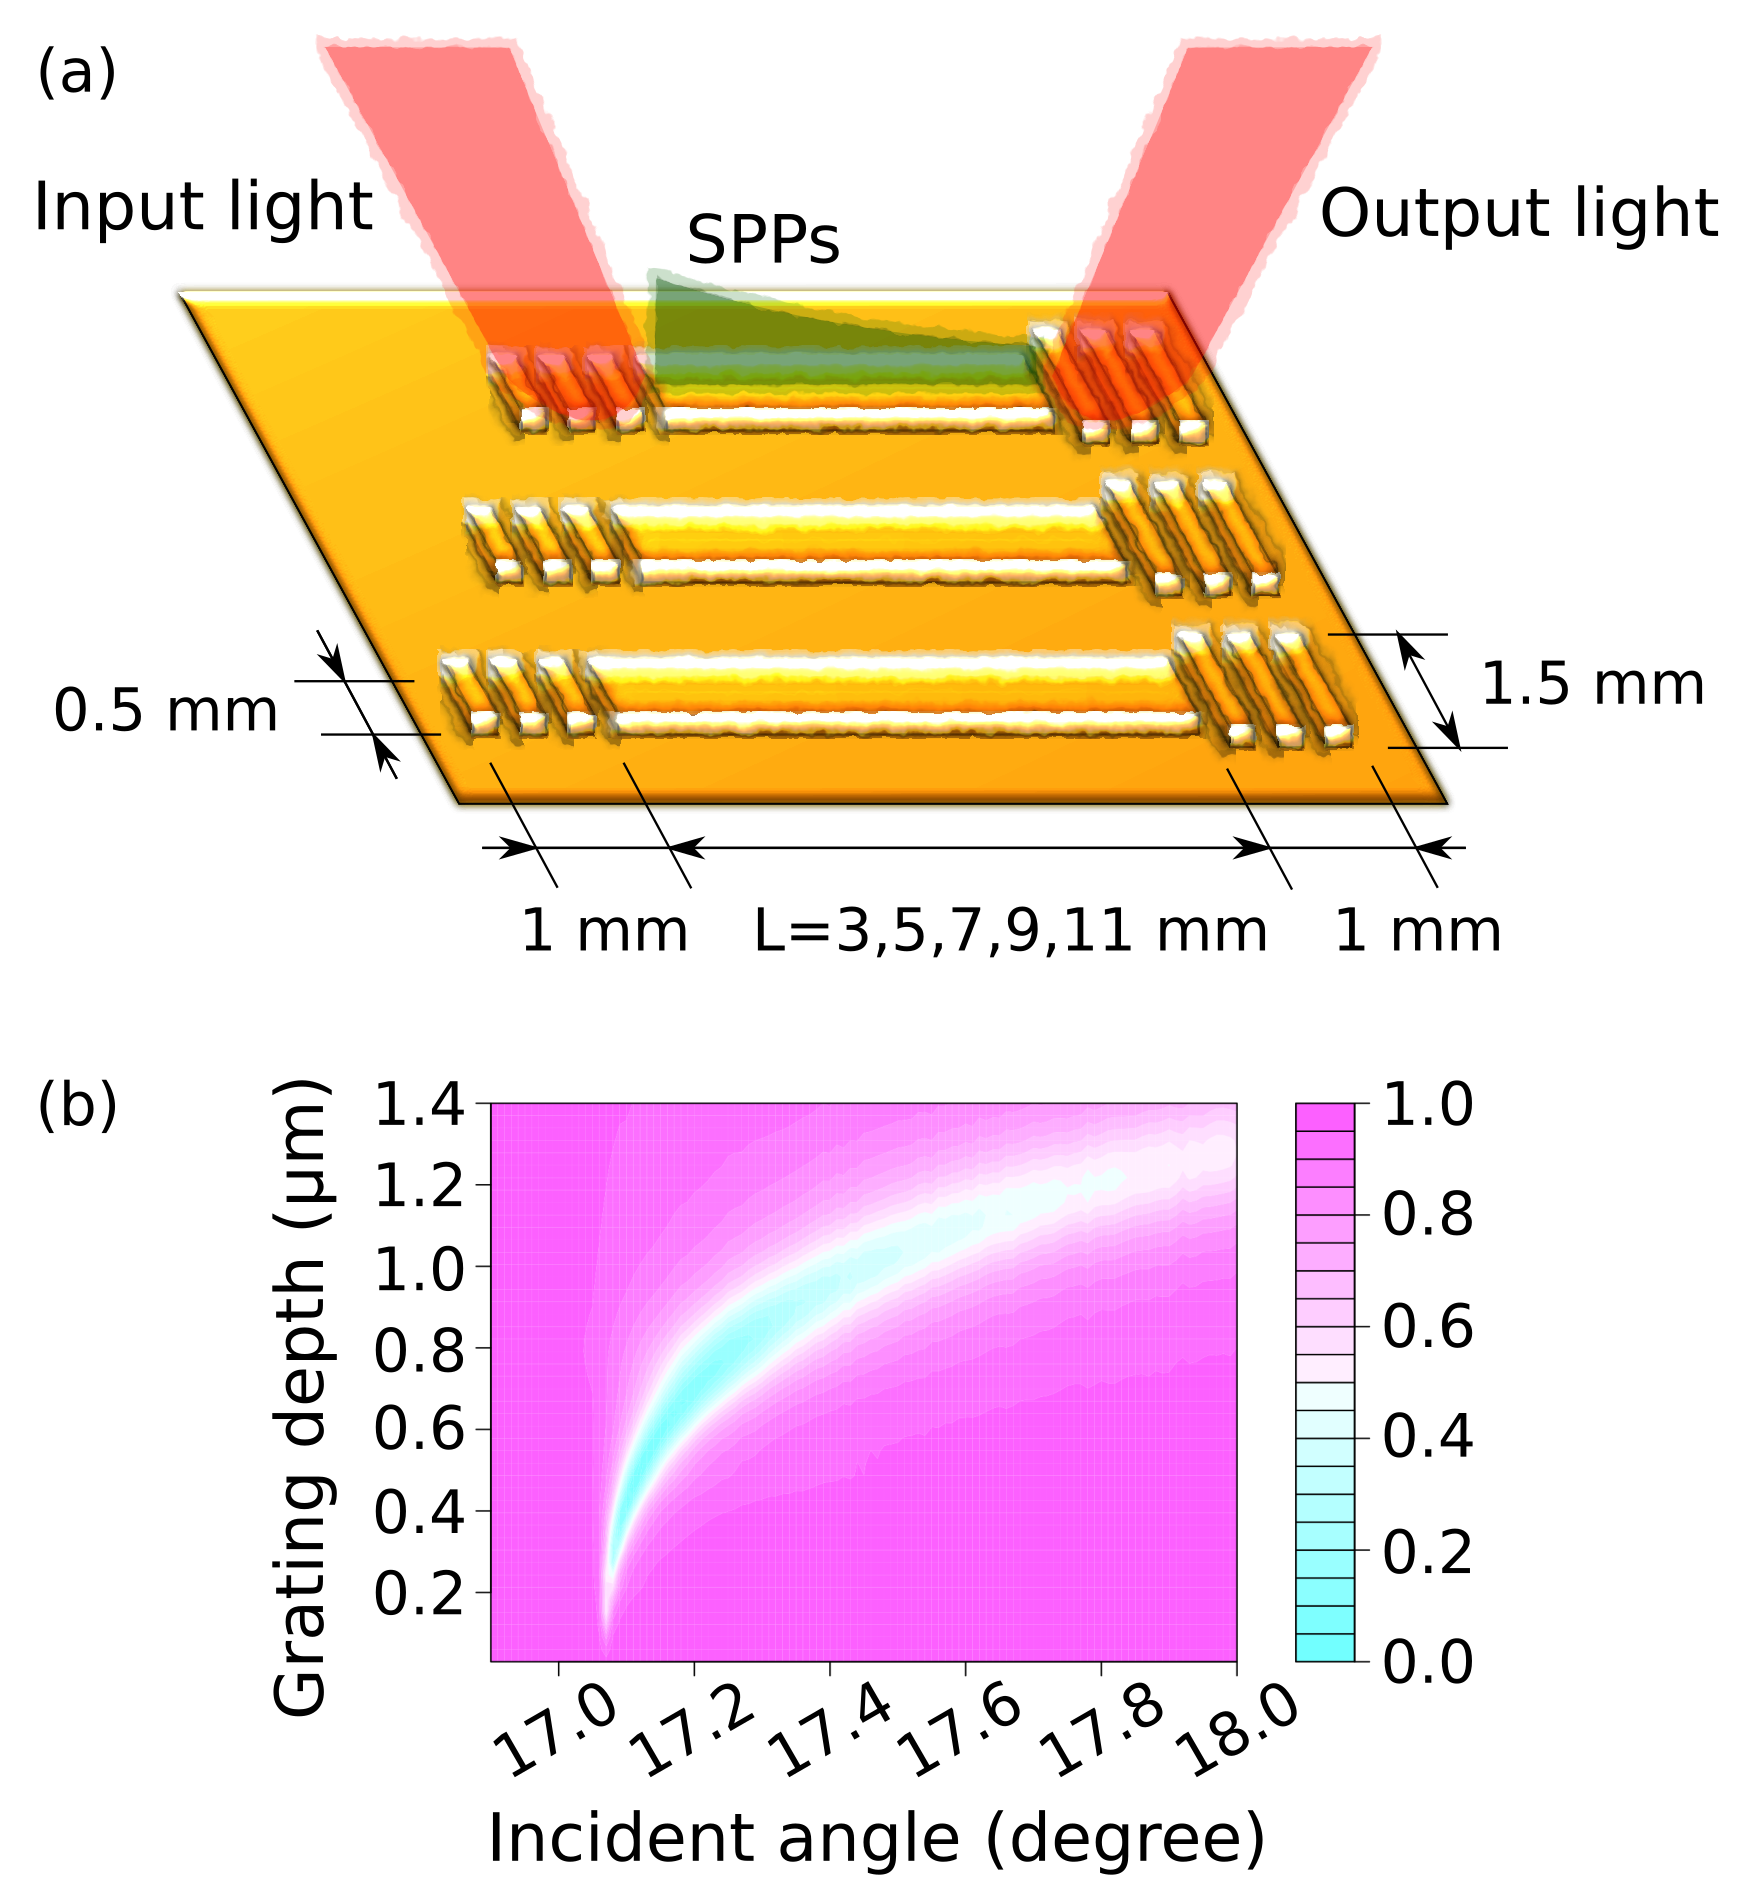
\includegraphics[width=0.8\hsize]{device.eps}
    \caption{(a) Schematic of the SPP waveguide devices. (b) Calculated reflection efficiency of a gold relief grating with a grating pitch of $15\:\mathrm{\mu m}$ and a duty cycle of 0.5, as a function of incident angle and grating depth.}
     \label{fig:device}
\end{figure}

\section{Experiment}
\label{sec:experiment}
Figure \ref{fig:experiment} shows the schematic of our experimental setup. 
A $\mathrm{CO_2}$ laser (L3SL, Access Laser Company) was used as a mid-IR light source generating linearly polarized light at a wavelength of $10.6\:\mathrm{\mu m}$. 
SPP devices were attached to a rotational and 3D-translational stage. 
The p-polarized light (electric field oscillates parallelly to the plane of incidence) was incident onto the input coupler at the angle that fulfills Eq. \ref{eq:phase-match} where $m=1$, being loosely focused by a spherical mirror with a curvature radius $R$ of $400\:\mathrm{mm}$.  Here the incident light converged with an angle of 1.3 degree to form the beam spot of $0.6\:\mathrm{mm}$ diameter at the sample position. This plane-like wavefront of the incident light and the homogeneous grating coupler should result in a SPP beam with plane-like wavefront. Because the focal depth of the excited SPP beam is $\sim10\:\mathrm{mm}$, and because the SPPs are confined in the waveguides, we ignored the propagation loss due to diffraction.
The output light was collected by a spherical mirror of $R=150\:\mathrm{mm}$ and a power meter. 
An aperture was placed at the conjugate point of the output coupler to avoid any stray light. 
Time-averaged power of the $\mathrm{CO_2}$ laser was controlled by changing the duty ratio of RF power modulation.
Typically, time-averaged optical power sent to the input coupler was $60\:\mathrm{mW}$, and the duty ratio was $0.5$. 

In order to modify the morphology of the gold film, the sample containing a series of waveguide devices was annealed twice with a hotplate in argon atmosphere\cite{Nogues}.
In the first annealing process, the sample was heated at $600\:^\circ\mathrm{C}$ for $20\:\mathrm{min}$., and gradually cooled down to room temperature on the hotplate. In the second annealing process, the sample was heated at $700\:^\circ\mathrm{C}$ for $16\:\mathrm{min}$., and cooled down in the same way. Surface morphology was measured by AFM (SPA-300, Seiko Instruments Inc.) in tapping mode.

 \begin{figure}
    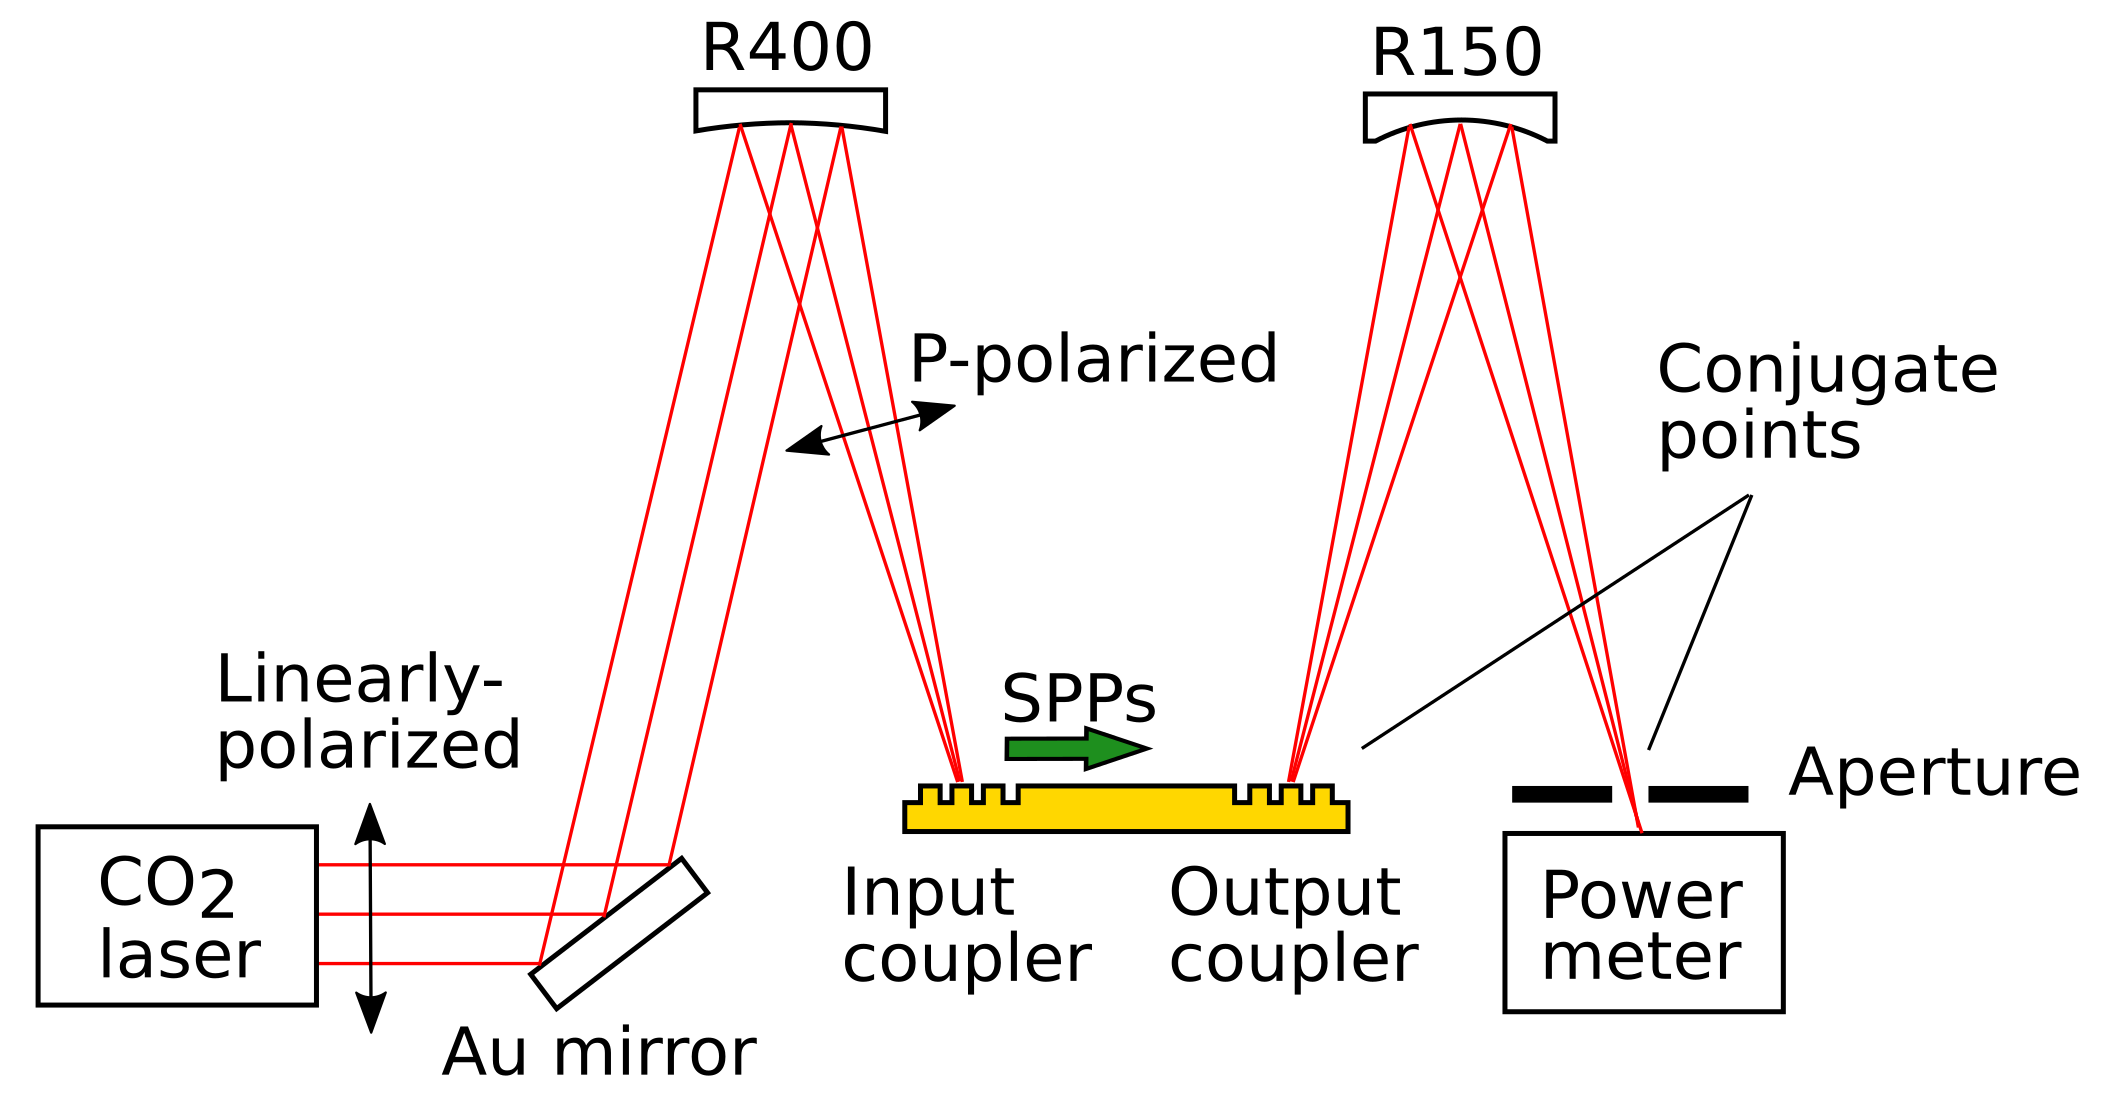
\includegraphics[width=0.85\hsize]{experiment.eps}
    \caption{Schematic of the experimental setup.}
     \label{fig:experiment}
\end{figure}

\section{Results}
\label{sec:result}
Figure \ref{fig:propagation_length} shows the measured output power as a function of the waveguide length $L$ for (a) as-grown, (b) once-annealed ($600\:^\circ\mathrm{C}$), and (c) twice-annealed ($600\:^\circ\mathrm{C}$ and $700\:^\circ\mathrm{C}$) samples.
Here, each trace is normalized by the value at $L=0$.
Each trace was fitted with the exponential decay function $\exp(-L/L_{\mathrm{SPP}})$, and the propagation length $L_{\mathrm{SPP}}$ was evaluated as $9.0\pm0.3\:\mathrm{mm}$, $12.0\pm0.4\:\mathrm{mm}$, and $14.7\pm0.7\:\mathrm{mm}$ for the as-grown, once-annealed, and twice-annealed samples, respectively.
In this way, the SPP propagation length increased by the annealing process.

Figure \ref{fig:morphology} shows AFM topography images of the waveguide surfaces (upper panels), and the cross-sectional height data (lower panels) for (a) as-grown, (b) once-annealed ($600\:^\circ\mathrm{C}$), and (c) twice-annealed ($600\:^\circ\mathrm{C}$ and $700\:^\circ\mathrm{C}$) samples. Here the sectional surface is indicated as dashed blue-lines in the topography images. The granular pattern typical for polycrystalline gold is clearly observed for the as-grown sample, as shown in Fig. \ref{fig:morphology}(a). Although the grain boundaries became unclear, the average grain size seemed to increase upon annealing, as shown in Fig. \ref{fig:morphology} (b,c),  We identified crystal grains and estimated their average size by analyzing the height data with the watershed algorithm\cite{Petr}. By assuming that each grain has spherical shape, grain diameter is estimated to be $70\pm20\:\mathrm{nm}$, $190\pm90\:\mathrm{nm}$, and $180\pm80\:\mathrm{nm}$ for the as-grown, once-annealed, and twice-annealed samples, respectively. It is evident from the cross-sectional height data shown in the lower panels in Figs. \ref{fig:morphology} (a-c) that surface roughness decreased upon annealing. By calculating root mean squares of deviations in height data, the surface roughness is estimated to be $5.7\:\mathrm{nm}$, $2.8\:\mathrm{nm}$, and $2.2\:\mathrm{nm}$ for the as-grown, once-annealed, and twice-annealed samples, respectively. In this way, the thermal annealing at $600\:^\circ\mathrm{C}$ or above was found to increase the grain size and reduce the surface roughness.

The SPP-light coupling efficiency of the coupler grating is estimated to be 0.18 in our experiments. Although optimum incident angle for the maximum coupling efficiency shifted by about $0.5^\circ$ upon annealing, the change in the maximum coupling efficiency was not observed. The AFM measurements confirmed that the coupler gratings had ideal rectangular profiles which did not change by the annealing treatments. 

 \begin{figure}
    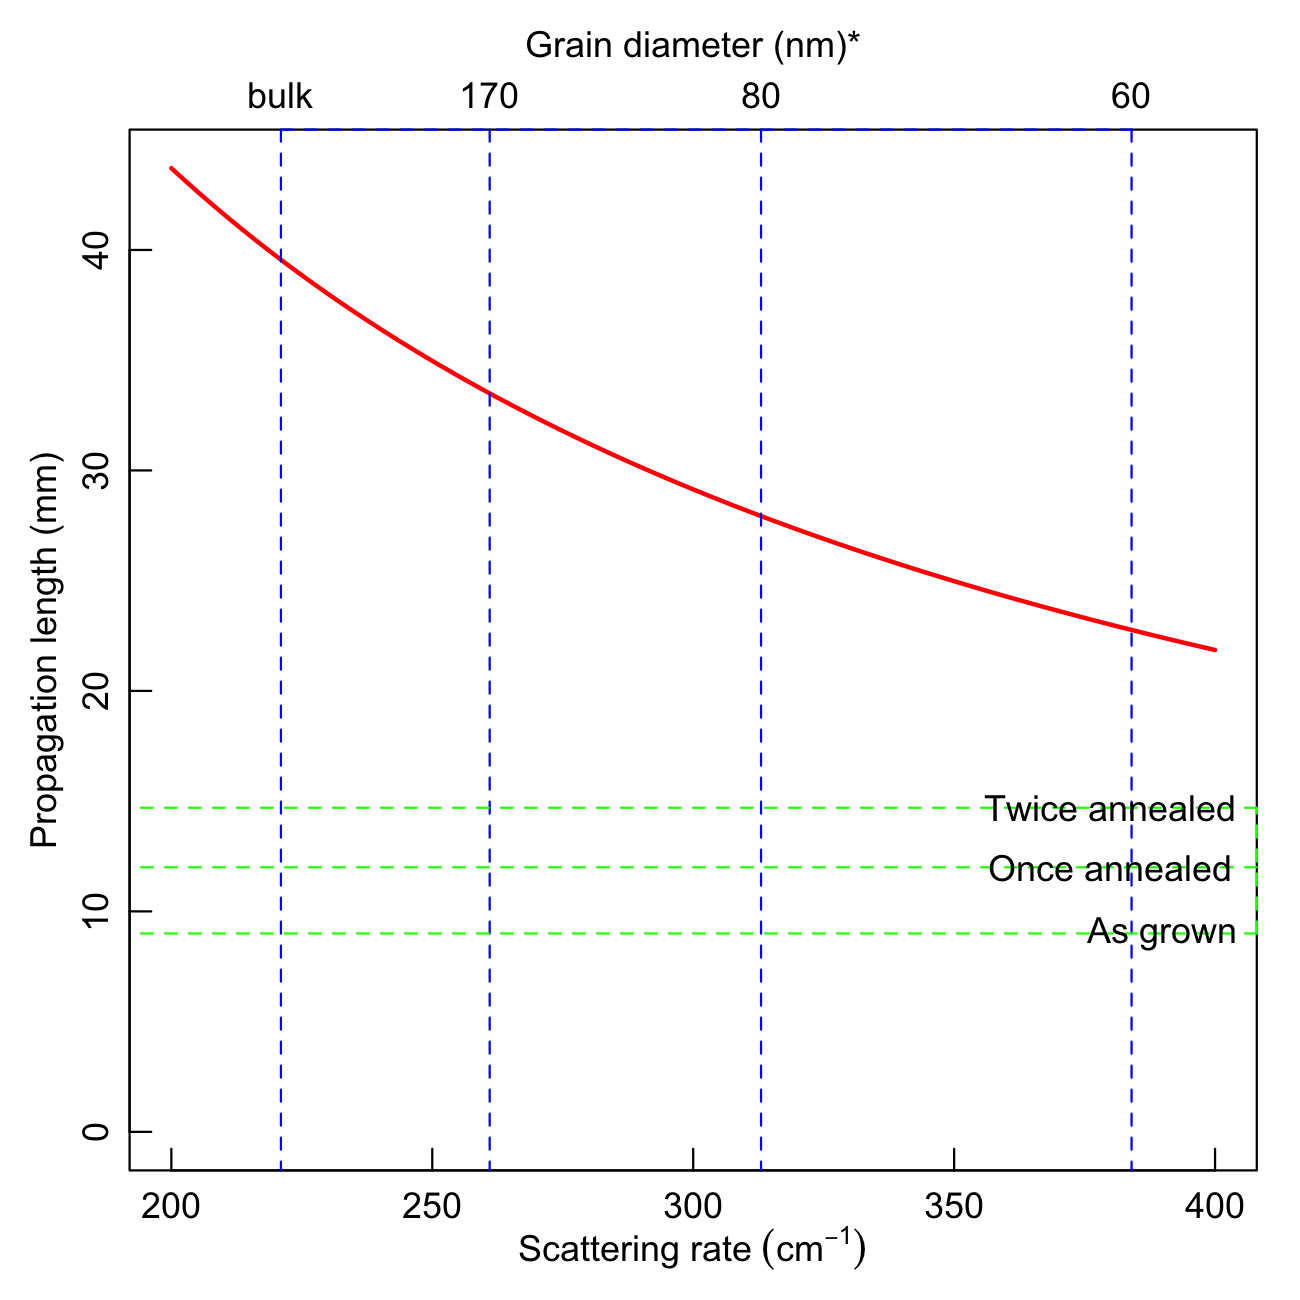
\includegraphics[width=0.85\hsize]{propagation_length.eps}
    \caption{Normalized output power as a function of the SPP waveguide length $L$ for (a) as-grown, (b) once-annealed ($600\:^\circ\mathrm{C}$), and (c) twice-annealed samples ($600\:^\circ\mathrm{C}$ and $700\:^\circ\mathrm{C}$). The propagation length of SPP is evaluated as $9.0\pm0.3\:\mathrm{mm}$, $12.0\pm0.4\:\mathrm{mm}$, and $14.7\pm0.7\:\mathrm{mm}$ for the sample (a), (b), and (c), respectively.}
       \label{fig:propagation_length}
\end{figure}

 \begin{figure}
    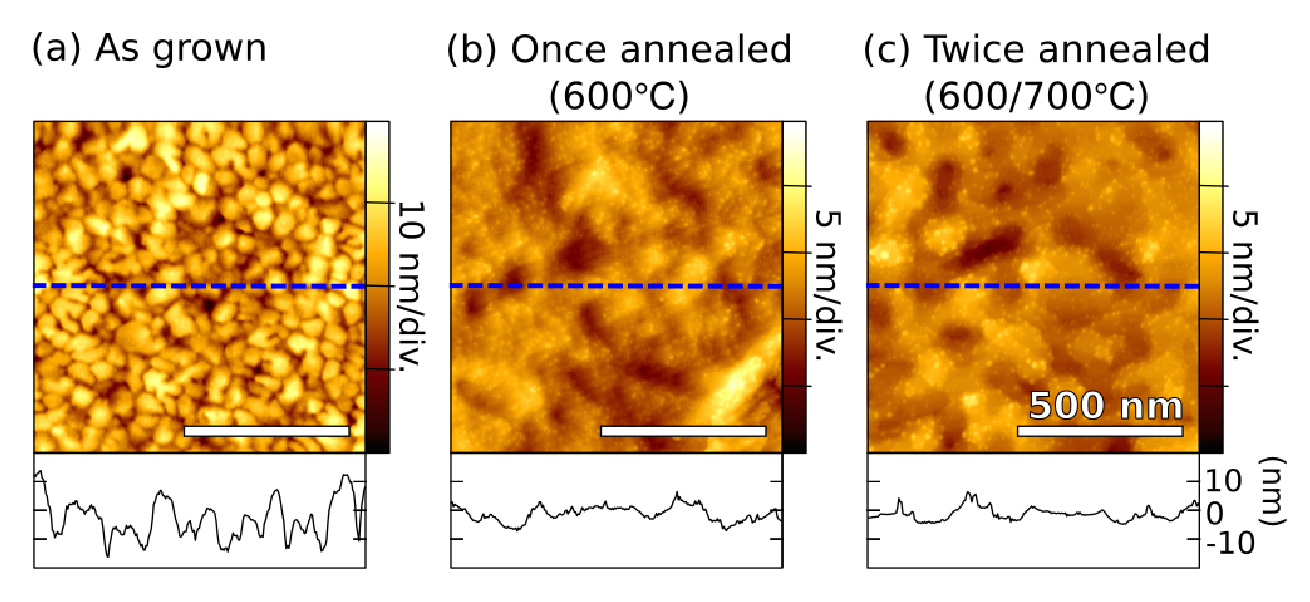
\includegraphics[width=\hsize]{morphology.eps}
    \caption{AFM topography images (upper panels) of the waveguide surface, and the cross-sectional height data (lower panels) for (a) as-grown, (b) once-annealed ($600\:^\circ\mathrm{C}$), and (c) twice-annealed ($600\:^\circ\mathrm{C}$ and $700\:^\circ\mathrm{C}$) samples. The sectional surface is indicated as blue dashed lines. }
    \label{fig:morphology}
\end{figure}

\section{Discussions}
\label{sec:discussion}
Considering only Ohmic losses, the SPP propagation length $L_{\mathrm{SPP}}$ at a metal/air interface is expressed by the following equation,
\begin{equation}
 L_{\mathrm{SPP}} = \frac{1}{2\:\mathrm{Im} k_{\mathrm{SPP}}},
\label{eq:propagation_length}
 \end{equation}
where $k_{SPP}=(\lambda/2\pi)\sqrt{\epsilon_g/(\epsilon_g+1)}$ is the complex wavenumber of the SPPs, and $\epsilon_g=\epsilon'_g+i\epsilon''_g$ is the relative dielectric constant of gold. 
By substituting the dielectric constant of polycrystalline gold\cite{Palik} into Eqn. \ref{eq:propagation_length}, the propagation length of SPP is calculated to be $12.3\:\mathrm{mm}$ at a wavelength of $10.6\:\mathrm{\mu m}$.
Our experimentally measured values of  $9.0\pm0.3\:\mathrm{mm}$, $12.0\pm0.4\:\mathrm{mm}$, and $14.7\pm0.7\:\mathrm{mm}$ agree with the theoretical estimation, confirming that mid-IR SPPs at gold/air interface propagates for a distance as long as $>10\:\mathrm{mm}$.

SPPs at planer metal/air interface decay mainly due to the Ohmic loss  (scattering of free electrons by electrons, phonons, defects, impurities, etc.) and partly due to scattering of SPPs by surface roughness, grain boundaries, etc\cite{Kuttge, Lee}. It has been suggested that the grain boundaries of polycrystalline gold reduce the mean free path of free electrons, and therefore increase the Ohmic loss\cite{Kuttge, Yang, Trollmann}.

In our experiments, the average grain size increased and the surface roughness decreased by the thermal annealing. Such morphology change can be understood as that smaller crystallite grains preferentially melt upon annealing\cite{Buffat} and then re-crystallize into larger particles. Reduced surface roughness, on the other hand, may imply that voids existing among crystallites were partly eliminated through the anneling treatments.  

The increase in SPP propagation length upon the first annealing was correlated with the increased grain size and the suppressed surface roughness. Here we can naturally conclude that the thermal annealing increased the grain size, which in turn reduced both the Ohmic loss and the SPP scattering loss. Suppressed surface roughness may also have reduced the scattering of SPPs to some extent. Simultaneous measurements on dielectric constants may help evaluating each contribution separately (reduced Ohmic loss and reduced SPP scattering). 

Upon the second thermal annealing at $700\:^\circ\mathrm{C}$, the SPP propagation length increased further, although the average grain size and the surface roughness did not show clear change. The reason for this further increase has not been clarified yet, but it may be due to the decrease in grain boundaries and voids. Such morphology change beneath the surface within a skin depth would affect the scattering of electrons and that of SPPs. 

As described above, we have successfully demonstrated that the simple treatment of thermal annealing leads to elongation of SPP propagation length, accmpanied by the morphology change characterized by the increased grain size and the reduced surface roughness. It has, however, minor side effect that pinholes may be generated on metal surface. In fact, pinholes with diameters of $<1\:\mathrm{\mu m}$ appeared with a number density of $0.16\:\mathrm{\mu m}^{-2}$ after the first annealing, and with a number density of $0.44\:\mathrm{\mu m}^{-2}$ after the second annealing. Such pinholes are much smaller than the SPP wavelength but may scatter SPPs. It would be safely concluded, however, that the increase of the propagation length due to morphology change was more than the decrease of the propagation length due to the pinholes.
	
\section{Conclusions}
\label{sec:conclusion}
We experimentally measured the propagation length of SPPs at gold/air interface in the mid-IR range. We confirmed that SPPs at gold/air interface propagate for a distance as long as $>10\:\mathrm{mm}$ at a wavelength of $10.6\:\mathrm{\mu m}$. The measured propagation length is in good agreement with the value predicted from the dielectric constant of polycrystalline gold. We successfully demonstrated that the SPP propagation length increases by the simple thermal annealing treatment, accompanied by the increased grain size and the suppressed surface roughness. Quantitative evaluation of the SPP propagation length, correlated with material's morphology, is important in designing plasmonic devices and beneficial for deeper understandings of the loss mechanism and the achievable electric-field enhancements of mid-IR SPs on gold.

\section*{Acknowledgement}
The author thank K. Hirakawa for technical supports in thermal evaporation and annealing, T. Takahashi and Y. Shimada for  technical support of AFM measuments.
The sample was fabricated at VLSI Design and Education Center (VDEC), the University of Tokyo. Finantial support by the Japan Society for the Promotion of Science (MEXT KAKENHI 16K13694) is gratefully achnowledged.

\bibliography{Reference}

\newpage

\end{document}